\scanpage{118}
\mspage{117}
\mspage{4}
\deleted{Soit} $i$

\deleted{L'introduction des $\Lambda_r^i$}

Fixons nous un indice dans $\{0,1,\infty\}$, disons $1$ (en pensant au cas où la triangulation est barycentrique, donc \inserted{où} $1$ joue un rôle particulier !). Nous pouvons éliminer les sommets $R_r^{ij}$ qui se trouvent sur des côtés de $r$ qui sont de type $1$, i.e. pour lesquels $i,j\ne1$, et l'arc $a_r^1$ qui les joint, en gardant les sommets
\[
(14)\qquad\left\{R_r^{i,j}\quad\left\{\begin{array}{l}
r\in\mathcal{R}\\
i\text{ ou }j\text{ est égal à }1\quad\text{i.e.}\quad\{i,j\}\ne\{0,\infty\}
\end{array}\right.\right.
\]
et les arcs
\[
(15)\qquad\left\{\begin{array}{ll}
\lambda_r^1&r\in\mathcal{R}\\
\Lambda_r^0,\Lambda_r^{\prime\infty}&r\in\mathcal{R},\quad\deleted{\unsure{i\in\{0,\infty\}}}\\
a_r^i&r\in\mathcal{R},\quad i\in\{0,\infty\}
\end{array}\right.
\]
\margin{$\Lambda_r^0\Lambda_{\tau_1r}^0=$}
avec comme relations les relations $(14)$ de redondance \inserted{pour $i=0$ et $i=\infty$} \deleted{\unsure{et les relations du type} $\unsure{\Lambda_r^0}=\unsure{1}$}
\deleted{
\[
\boxed{
\Lambda_{\tau_1r}^{\unsure{\infty|\prime\infty}}
\underbrace{(a_{\tau_1r}^0(\lambda_{\tau_1r}^1)^{-1}a_{\tau_1r}^\infty)^{-1}}_{\beta_{\tau_1r}^{1\,-1}}
\Lambda_r^0\underbrace{a_r^\infty\lambda_r^1a_r^0}_{\unsure{\beta_r^1}}=1
}\qquad(16)
\]
pour $r\in\mathcal{R}$ (lacets en $R_r^{01}$)

\uline{NB} Cette relation est équivalente à la relation \deleted{\unsure{inverse}} \inserted{où $r$ est remplacé} par $\unsure{\sigma_1r|\tau_1r}$
}

\margin{pavage par des carrés ? (dont les sommets \unsure{qui ne sont} pas de type $1$, sont ``arrondis'', de façon à faire des hexagones \unsure{évitant} les trous}
\figure{
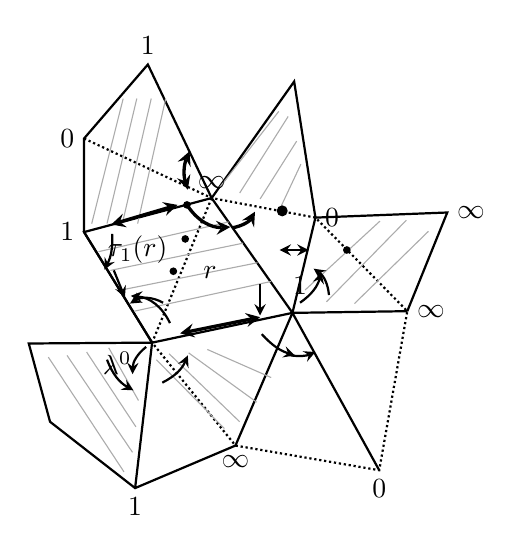
\begin{tikzpicture}[scale=1.08,>=stealth]
\coordinate (A) at (1.25,1.85);\coordinate (B) at (2.90,2.20);\coordinate (C) at (1.95,3.55);
\coordinate (D) at (0.45,3.15);\coordinate (E) at (0.45,4.25);\coordinate (F) at (1.20,5.12);
\coordinate (G) at (2.92,4.92);\coordinate (H) at (3.17,3.32);\coordinate (I) at (4.72,3.38);
\coordinate (J) at (4.25,2.22);\coordinate (K) at (3.92,0.35);\coordinate (L) at (2.23,0.64);
\coordinate (M) at (1.05,0.14);\coordinate (N) at (0.05,0.92);\coordinate (O) at (-0.20,1.84);
\draw[thick] (D)--(E)--(F)--(C) (C)--(G)--(H) (H)--(I)--(J) (B)--(J);
\draw[thick] (B)--(K) (B)--(L)--(M)--(N)--(O)--(A) (A)--(M) (A)--(D);
\draw[densely dotted,thick] (E)--(C)--(H)--(J)--(K)--(L)--(A)--(C);
\draw[thick] (D)--(C)--(B)--(A)--cycle (B)--(H);
\foreach \p/\q in {0.54/0.91,0.72/1.07,0.90/1.24,1.08/1.41}{\draw[gray!65] (\p,3.25)--(\q,4.72);}
\draw[gray!65] (2.04,3.67)--(2.74,4.57) (2.28,3.61)--(2.85,4.51) (2.52,3.54)--(2.95,4.22) (2.77,3.46)--(3.00,3.95);
\draw[gray!65] (3.05,2.47)--(3.93,3.28) (3.30,2.33)--(4.24,3.29) (3.63,2.31)--(4.50,3.16);
\draw[gray!65] (0.62,2.92)--(2.15,3.27) (0.76,2.70)--(2.32,3.02) (0.89,2.47)--(2.49,2.79) (1.04,2.22)--(2.65,2.57);
\draw[gray!65] (1.30,1.65)--(2.10,0.84) (1.45,1.72)--(2.28,0.92) (1.68,1.73)--(2.48,1.15) (1.90,1.77)--(2.65,1.44);
\draw[gray!65] (0.03,1.68)--(0.92,0.33) (0.25,1.70)--(1.02,0.56) (0.48,1.74)--(1.06,0.86) (0.74,1.79)--(1.09,1.17);
\fill (2.78,3.40) circle (0.065);\fill (1.66,3.47) circle (0.045);\fill (1.64,3.07) circle (0.045);\fill (1.50,2.69) circle (0.045);\fill (3.54,2.94) circle (0.045);
\draw[very thick,<->] (0.77,3.24)--(1.55,3.47);
\draw[very thick,<->] (1.67,3.65) to[bend left=20] (1.69,4.10);
\draw[very thick,->] (1.66,3.47) to[bend right=30] (2.17,3.21);
\draw[very thick,->] (2.19,3.20) to[bend right=25] (2.46,3.39);
\draw[thick,->] (0.78,3.13) to[bend left=15] (0.69,2.71);
\draw[thick,->] (0.80,2.70)--(0.93,2.38);
\draw[thick,->] (1.46,2.08) to[bend right=30] (1.00,2.40);
\draw[thick,->] (1.38,2.32) to[bend right=30] (0.99,2.31);
\draw[very thick,<->] (1.58,1.96)--(2.52,2.15);
\draw[thick,->] (2.52,2.54)--(2.52,2.17);
\draw[thick,<->] (2.75,2.94)--(3.09,2.94);
\draw[thick,->] (2.99,2.32) to[bend right=20] (3.24,2.68);
\draw[thick,->] (3.33,2.41) to[bend right=25] (3.15,2.72);
\draw[thick,->] (2.54,1.95) to[bend right=15] (2.93,1.70);
\draw[thick,->] (2.88,1.70) to[bend right=15] (3.17,1.74);
\draw[thick,->] (1.18,1.80) to[bend right=25] (1.02,1.48);
\draw[thick,->] (1.37,1.38) to[bend right=20] (1.67,1.70);
\draw[thick,->] (0.72,1.65) to[bend right=20] (1.03,1.29);
\node[above] at (F) {$1$};\node[left] at (E) {$0$};\node[left] at (D) {$1$};\node[above] at (C) {$\infty$};
\node[right] at (H) {$0$};\node[right] at (I) {$\infty$};\node[right] at (J) {$\unsure{\infty}$};\node[below] at (K) {$0$};
\node[below] at (L) {$\infty$};\node[below] at (M) {$1$};\node at (2.99,2.52) {$1$};
\node at (1.93,2.67) {$r$};\node at (1.08,2.94) {$\tau_1(r)$};\node at (0.84,1.61) {$\lambda^0$};
\end{tikzpicture}
}
\[
(16)\qquad\boxed{
\Lambda_{\tau_1(r)}^{\prime\infty}
\underbrace{(a_{\tau_1r}^0(\lambda_{\tau_1r}^1)^{-1}a_{\tau_1r}^\infty)^{\unsure{+|-1}}}_{\beta_{\tau_1(r)}^1\,\deleted{\unsure{-1}}}
\Lambda_r^0
\underbrace{((a_r^\infty)^{-1}\lambda_r^1(a_r^0)^{-1})}_{\beta_r^{1\,-1}}
=1
}
\]
\margin{relation stable par passage de $r$ à $\tau_1(r)$, donc il suffit de la poser pour $r\in\mathcal{R}^+$ (si $X$ orientable)}
\figure{
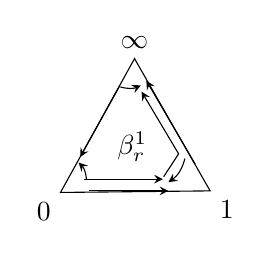
\begin{tikzpicture}[scale=1.0,>=stealth]
\coordinate (A) at (0,0);\coordinate (B) at (1.9,0.02);\coordinate (C) at (0.94,1.7);
\draw (A)--(B)--(C)--cycle;
\draw[->] (0.75,1.35)--(0.25,0.45);\draw[->] (0.36,0.02)--(1.37,0.02);\draw[->] (1.71,0.36)--(1.09,1.42);
\draw[->] (0.30,0.17)--(1.30,0.17);\draw[->] (1.31,0.20)--(1.50,0.49)--(1.03,1.28);
\draw[->] (0.76,1.34) to[bend right=20] (1.02,1.36);\draw[->] (0.33,0.16) to[bend right=20] (0.23,0.38);
\draw[->] (1.58,0.43) to[bend left=20] (1.37,0.13);
\node[below left] at (A) {$0$};\node[below right] at (B) {$1$};\node[above] at (C) {$\infty$};\node at (0.91,0.58) {$\beta_r^1$};
\end{tikzpicture}
}
